We designed a controller for an EUV (Extreme Ultra Violet) ASML waferstepper. This controller takes care of the logistics of silicon wafers in the waferstepper. If a rack of wafers arrives at an EUV waferstepper, they must enter the machine one by one through a sluice. There are two sluices, such that if one of the two sluices does not function the other can be used to let wafers enter and leave the machine.

There is one robot which picks wafers from the input rack and puts them into one of the two sluices. There is another robot inside the machine which takes wafers from the sluices and puts them into a waiting rack. A third robot moves the wafers from the waiting rack to the image projection system and moves them back to another waiting rack after an image has been projected. The wafers are subsequently moved through a sluice to the outside of the machine and to an output rack. The layout of the waferstepper is shown in figure~\ref{fig:stepperlayout}.

\begin{figure}[h]
    \centering
	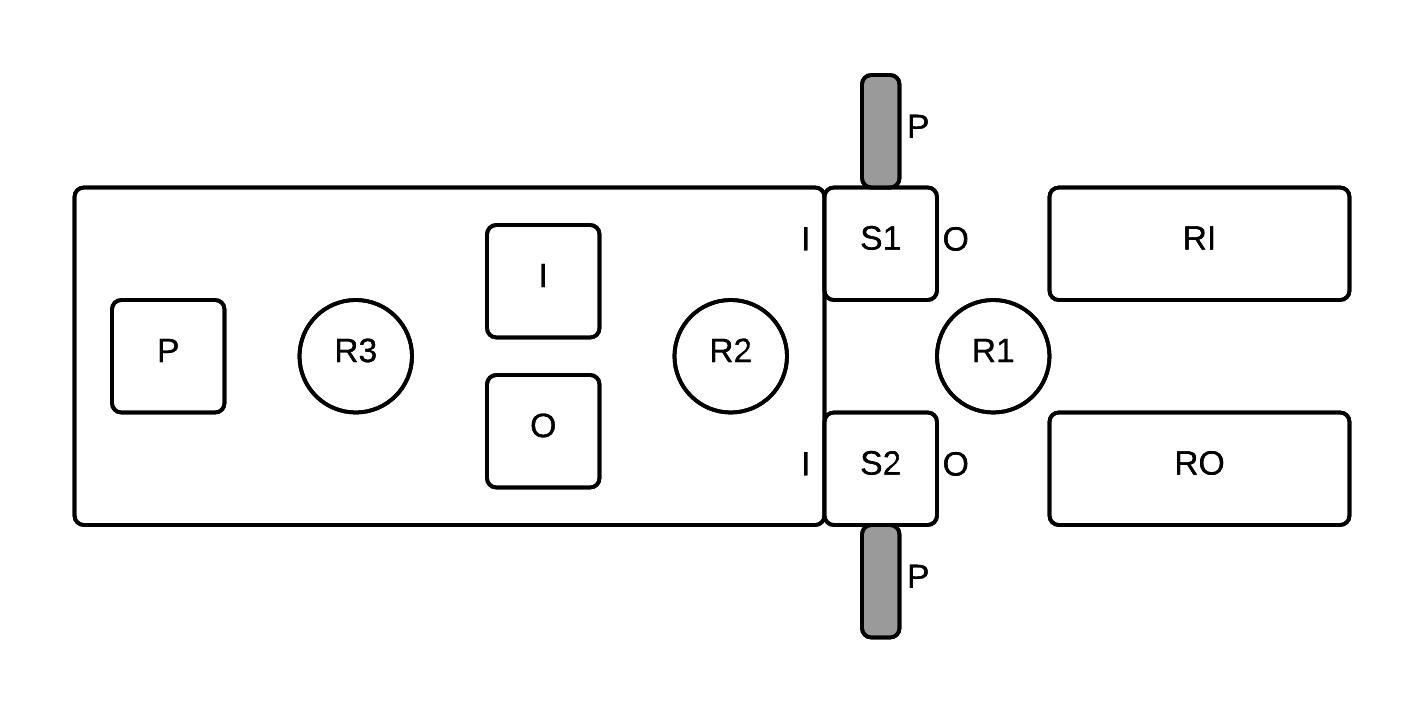
\includegraphics[width=0.6\textwidth]{waferstepper.png}
	\caption{The layout of the waferstepper.\\
	P: Projector\\R3: Robot that places wafers under the projector\\
	I: Waiting rack for unprocessed wafers\\
	O: Waiting rack for processed wafers\\
	R2: Robot that moves wafers from sluices to the waiting racks and vice versa\\
	S1 and S2: Sluices, each sluice has an inside door I, an outside door O and a pump P\\
	R1: Robot that moves wafers from the input rack to the sluices and from the sluices to the output rack\\
	RI: Wafer input rack\\
	RO: Wafer output rack}
	\label{fig:stepperlayout}
\end{figure}

The controller we design may not in any case perform harmful actions causing damage to the expensive waferstepper. The controller may not, for example, place wafers into a sluice when its doors are closed. Similarly it may not pick a wafer from a sluice with closed doors or from the projector while the wafer is begin projected. Additionally the controller should not place wafers on top of each other.

The doors of the sluices are less reliable and can get stuck. This is not something the controller can prevent, so it has to deal with broken doors and continue to operate even when a sluice is out of order. When this happens, the other sluice must be used to move wafers both into as out of the machine.